% !TEX root = ../../../main.tex
% 来源：中学数学实验教材·第二册（几何）
% 章节：实验几何 / 点、直线和平面
% 原始文件：1.tex，行 712-731
% 类型：tikz
% ---
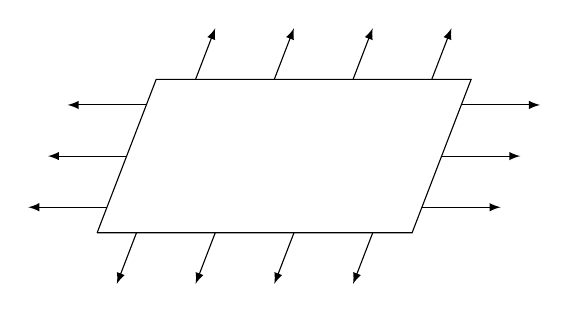
\begin{tikzpicture}[>=latex, yscale=1.5, x={(0:1cm)}, y={(60:.5cm)}]

\draw (0,0)--(4,0)--(4,3)--(0,3)--(0,0);
\foreach \x in {.5,1.5,...,3.5}
{
	\draw[->](\x,0)--(\x,-1);
	\draw[->](\x,3)--(\x,4);
}
\foreach \x in {.5,1.5,2.5}
{
	\draw[->](0,\x)--(-1,\x);
	\draw[->](4,\x)--(5,\x);
}

\tkzDefPoints{1/2.2/A, 2.8/.75/B}
\tkzDrawLine(A,B)
\tkzDrawPoints(A,B)
\tkzLabelPoints[right](A,B)

    \end{tikzpicture}
